\begin{answer}
	\begin{figure}[H]
	\centering
	\begin{subfigure}[H]{0.45\linewidth}
		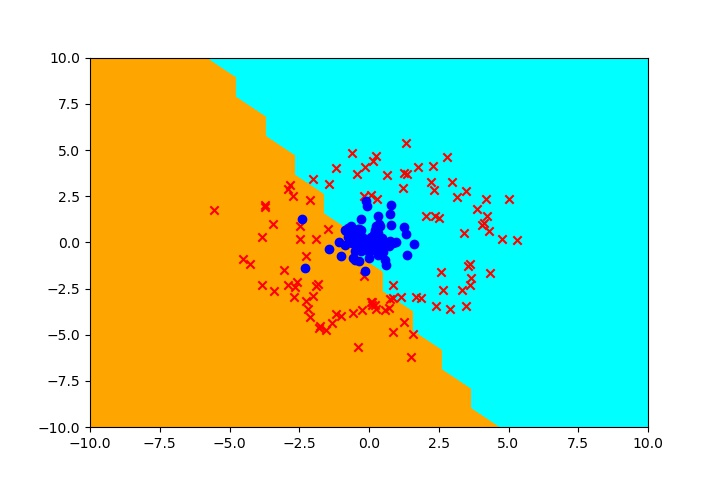
\includegraphics[width=\linewidth]{perceptron_dot_output}
		\caption{Dot-product kernel.}
	\end{subfigure}
	\begin{subfigure}[H]{0.45\linewidth}
		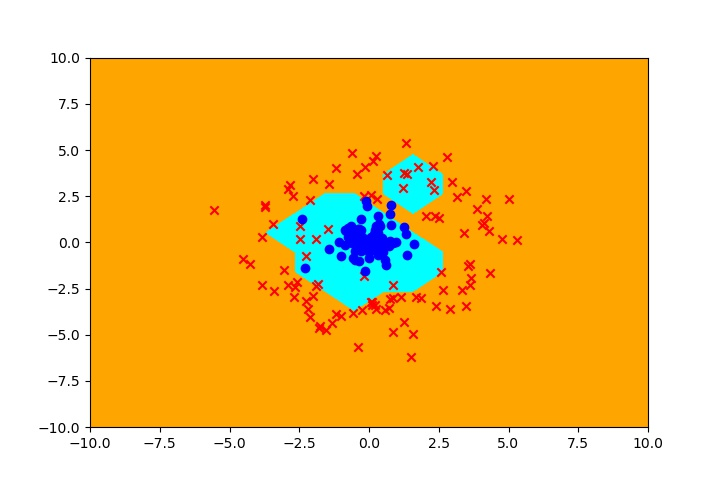
\includegraphics[width=\linewidth]{perceptron_rbf_output}
		\caption{RBF kernel.}
	\end{subfigure}
	\begin{subfigure}[H]{0.45\linewidth}
		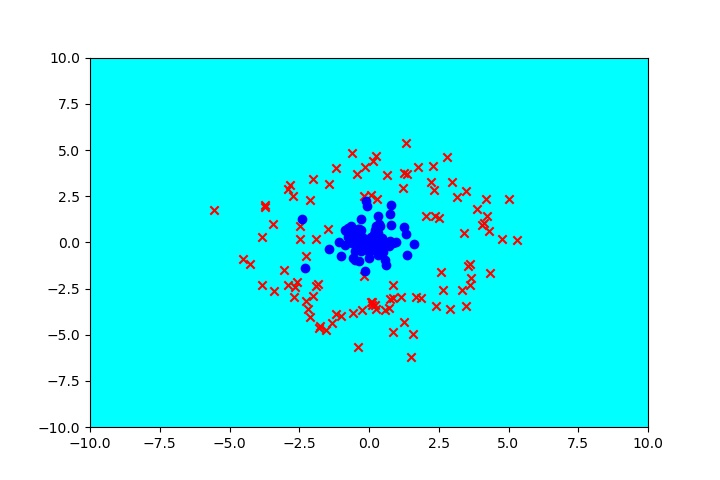
\includegraphics[width=\linewidth]{perceptron_non_psd_output}
		\caption{Not-a-kernel function.}
	\end{subfigure}
	\caption{The Perceptron using different kernels.}
	\end{figure}
\end{answer}
